\newpage
\subsection{Optimization results}  
In this section, we present the outcomes of the optimization studies on the Model 1 configuration using the Nelder--Mead and MADS methods. The objective functions considered are the near-wall shear rate and the turbulent kinetic energy. Our primary goals are to evaluate the convergence behavior of both optimization techniques, compare their efficiency, and assess their associated computational costs. Details of the hardware used for these computations can be found in \cite{gpu}.

The custom Nelder--Mead implementation was parallelized and executed on four dedicated compute nodes, managed through a Slurm-based job submission system \cite{slurm}. This setup enabled multiple function evaluations to be performed simultaneously, thereby reducing the total wall time for the optimization process. In contrast, the MADS method was not parallelized and thus ran sequentially on single-node configurations.

To ensure that the optimized configurations remained physiologically meaningful, we imposed constraints on the offset parameter \(o_1\). First, a primary geometrical constraint defined the feasible offset range as \(0{,}0 \leq o_1 \leq 2{,}4\,\text{cm}\). Next, to achieve the clinically motivated target that at least 25\% of the inferior vena cava (IVC) blood flow must be directed into the left pulmonary artery (LPA), we refined the constraint further. Using precomputed postprocessing analyses to identify offsets that satisfied this flow distribution, the offset was ultimately constrained to \(0{,}0 \leq o_1 \leq 0{,}78\,\text{cm}\), as shown in Figure~\ref{fig:ivc_flow_split}. Note that this approach contrasts with the optimization setup in Section~\ref{optim2}, where the IVC flow split is directly incorporated into the computations rather than relying on precomputed feasibility ranges.

Finally, the initial starting point for the optimization was chosen at the center of the feasible design space, \(o_1^\text{init} = 0{,}39\,\text{cm}\). Selecting a midpoint as the initial guess is a common practice to ensure that the optimizer explores the search space efficiently from a neutral starting position.

\vspace{7mm}
\begin{table}[H]
	\bgroup
	\centering
	\setlength\tabcolsep{3mm}
	\def\arraystretch{2.2}%
	\begin{tabular}{|c|c|c|}
		\hline
		\textbf{Method} & \textbf{Objective function} & \textbf{Page} \\ \hline
		Nelder-Mead & $\dot{\gamma}^{A}_{\mathrm{nw}}$ &\hyperlink{page.61}{61} \\ \hline
		Nelder-Mead & $T^{A}_{\mathrm{turb}}$ & \hyperlink{page.62}{62} \\ \hline
		MADS & $\dot{\gamma}^{A}_{\mathrm{nw}}$ & \hyperlink{page.63}{63} \\ \hline
		MADS & $T^{A}_{\mathrm{turb}}$ & \hyperlink{page.64}{64} \\ \hline
	\end{tabular}
	\caption{Key offset points selected for detailed analysis. Each point corresponds to notable extrema or special configurations of $\dot{\gamma}^{A}_{\mathrm{nw}}$ or $T^{A}_{\mathrm{turb}}$.}
	\label{tab:optim configs}
	\egroup
\end{table}

\newpage
\begin{optimproblem}{Basic cylindrical junction ($\dot{\gamma}^{A}_{\text{nw}}$)}
	\vspace{2mm}
	Objective:  Minimizing near-wall shear rate $\dot{\gamma}^{A}_{\text{nw}}$.
	
	\vspace{2mm}
	Geometrical model:
	\begin{itemize}
		\item Model 1 as described in Section~\ref{mod:model1}.
		\item Optimization parameters: offset $o_1$.
	\end{itemize}
	Constraints:
	\begin{itemize}
		\item Offset constraint: $0{,}0~\text{cm} \leq o_1 \leq 2{,}4~\text{cm}$.
		\item Flow split constraint: $F^{\text{LPA}}_{\text{IVC}} \geq 25~\%$.
	\end{itemize}
	Optimization method:
	\begin{itemize}
		\item Nelder-Mead method as described in Section~\ref{framework} and Appendix~\ref{appendix C}.
	\end{itemize}
	Initial point: $o^{\text{init}}_{1}$ = 0{,}39 cm
	\label{optimprob:1}
\end{optimproblem}
\vspace{-5mm}

\begin{figure}[H]
	\centering
	\begin{subfigure}{0.46\textwidth}
		\centering
		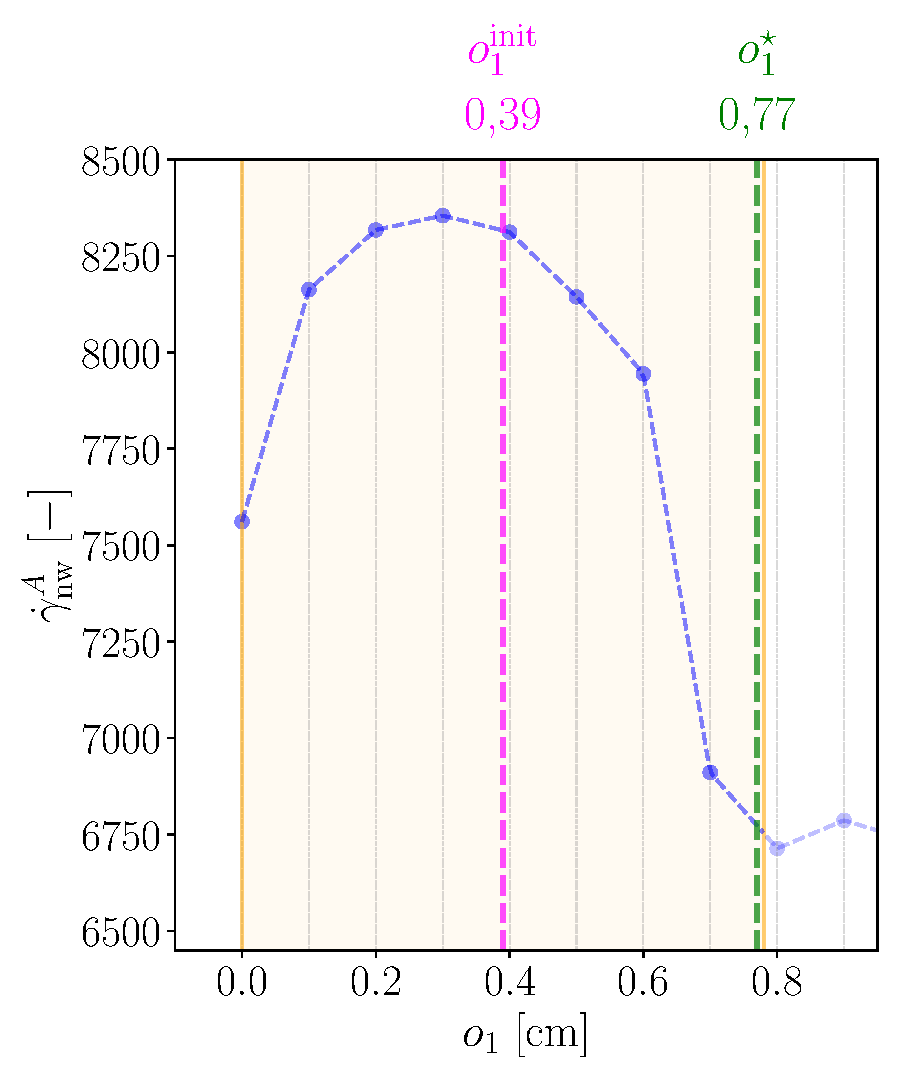
\includegraphics[
		width=\textwidth,
		trim={0mm 0mm 0mm -13mm}, clip
		]{figures/mean_stress_3_interpolated_point.pdf}
	\end{subfigure}\hfill%
	\begin{subfigure}{0.52\textwidth}
		\centering
		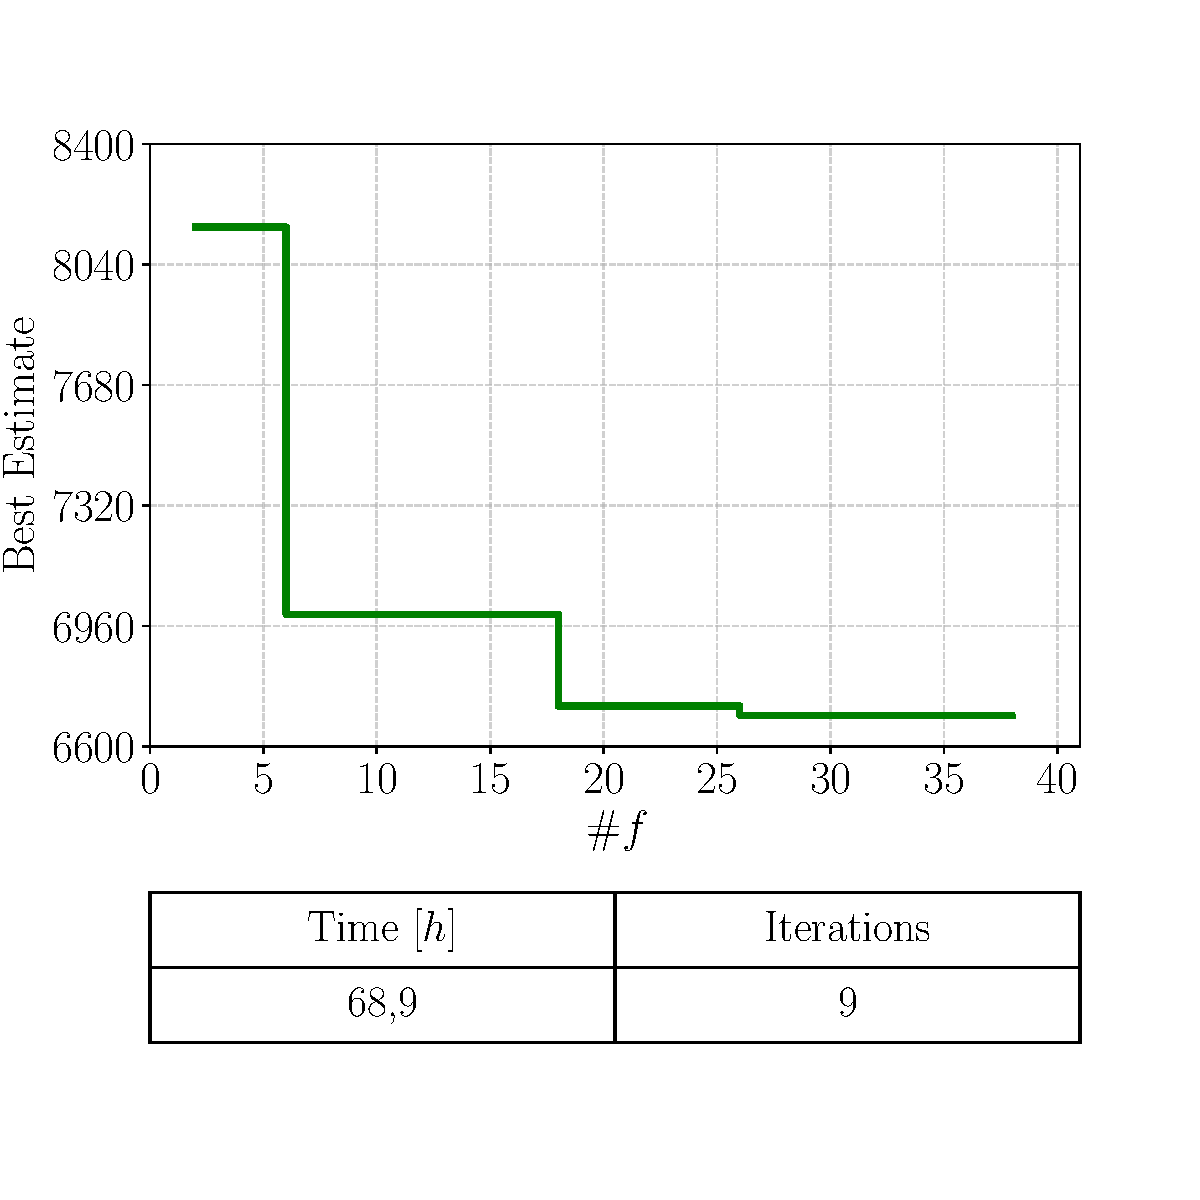
\includegraphics[
		width=1.05\textwidth,
		trim={0mm 25mm 0mm 0mm}, clip
		]{figures/optim_results/nm_sr.pdf}
	\end{subfigure}
	\vspace{2mm}
	\caption{Optimization results for Optimization Setup 1. The left plot compares the optimization result (marked point) with the previously sampled and interpolated objective function $\dot{\gamma}_{\text{max}}^{A}$ as a function of the parameter $o_1$. The right plot demonstrates the convergence of the optimization method, showing the best estimate against the number of objective function evaluations ($\# f$). The table summarizes the total elapsed time of the optimization algorithm (68,9 hours) and the number of iterations of the used method (9).}
\end{figure}
\newpage
\begin{optimproblem}{Basic cylindrical junction ($T^{A}_{\mathrm{turb}}$)}
	\vspace{2mm}
	Objective: Minimizing turbulent kinetic energy $T^{A}_{\mathrm{turb}}$.
	
	\vspace{2mm}
	Geometrical model:
	\begin{itemize}
		\item Model 1 as described in Section~\ref{mod:model1}.
		\item Optimization parameters: offset $o_1$.
	\end{itemize}
	Constraints:
	\begin{itemize}
		\item Offset constraint: $0{,}0~\text{cm} \leq o_1 \leq 2{,}4~\text{cm}$.
		\item Flow split constraint: $F^{\text{LPA}}_{\text{IVC}} \geq 25~\%$.
	\end{itemize}
	Optimization method:
	\begin{itemize}
		\item Nelder-Mead method as described in Section~\ref{framework} and Appendix~\ref{appendix C}.
	\end{itemize}
	Initial point: $o^{\text{init}}_{1}$ = 0{,}39 cm
	\label{optimprob:2}
\end{optimproblem}
\vspace{-5mm}

\begin{figure}[H]
	\centering
	\begin{subfigure}{0.46\textwidth}
		\centering
		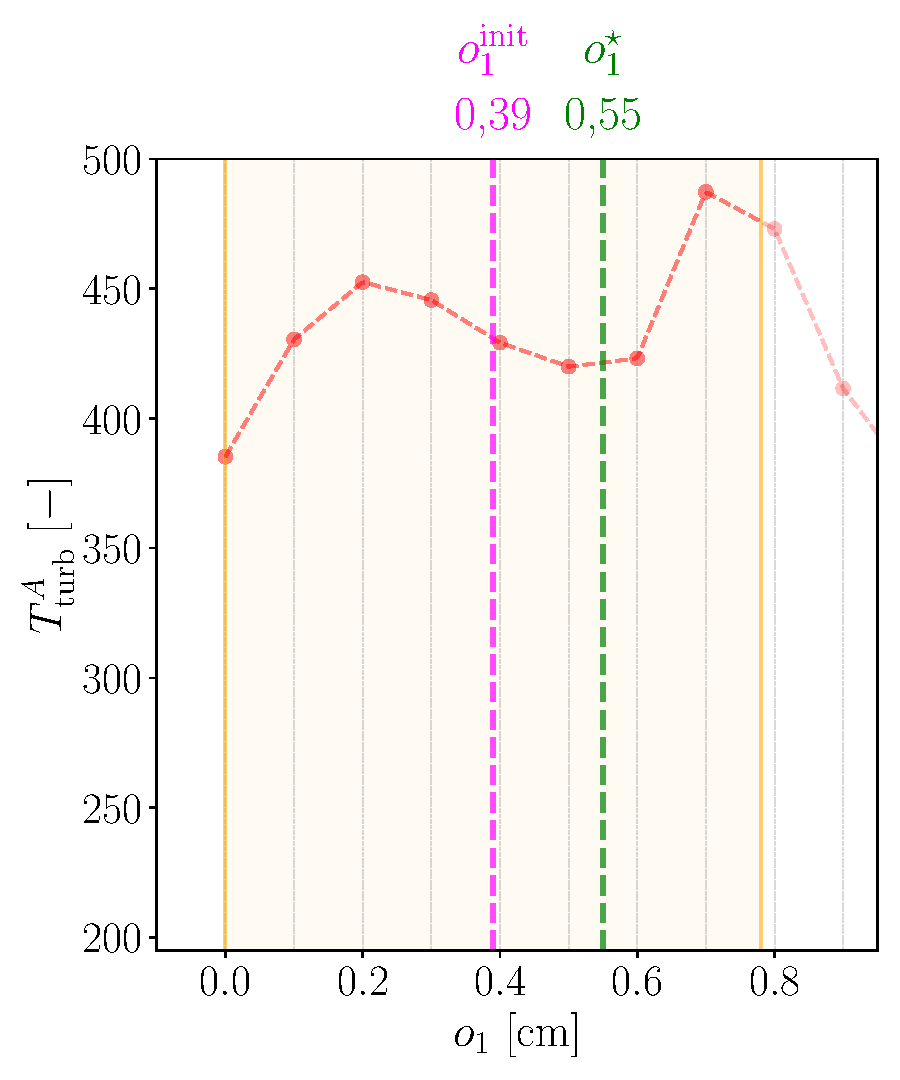
\includegraphics[
		width=\textwidth,
		trim={0mm 0mm 0mm -13mm}, clip
		]{figures/mean_turbulence_kinetic_energy_interpolated_point.pdf}
	\end{subfigure}\hfill%
	\begin{subfigure}{0.52\textwidth}
		\centering
		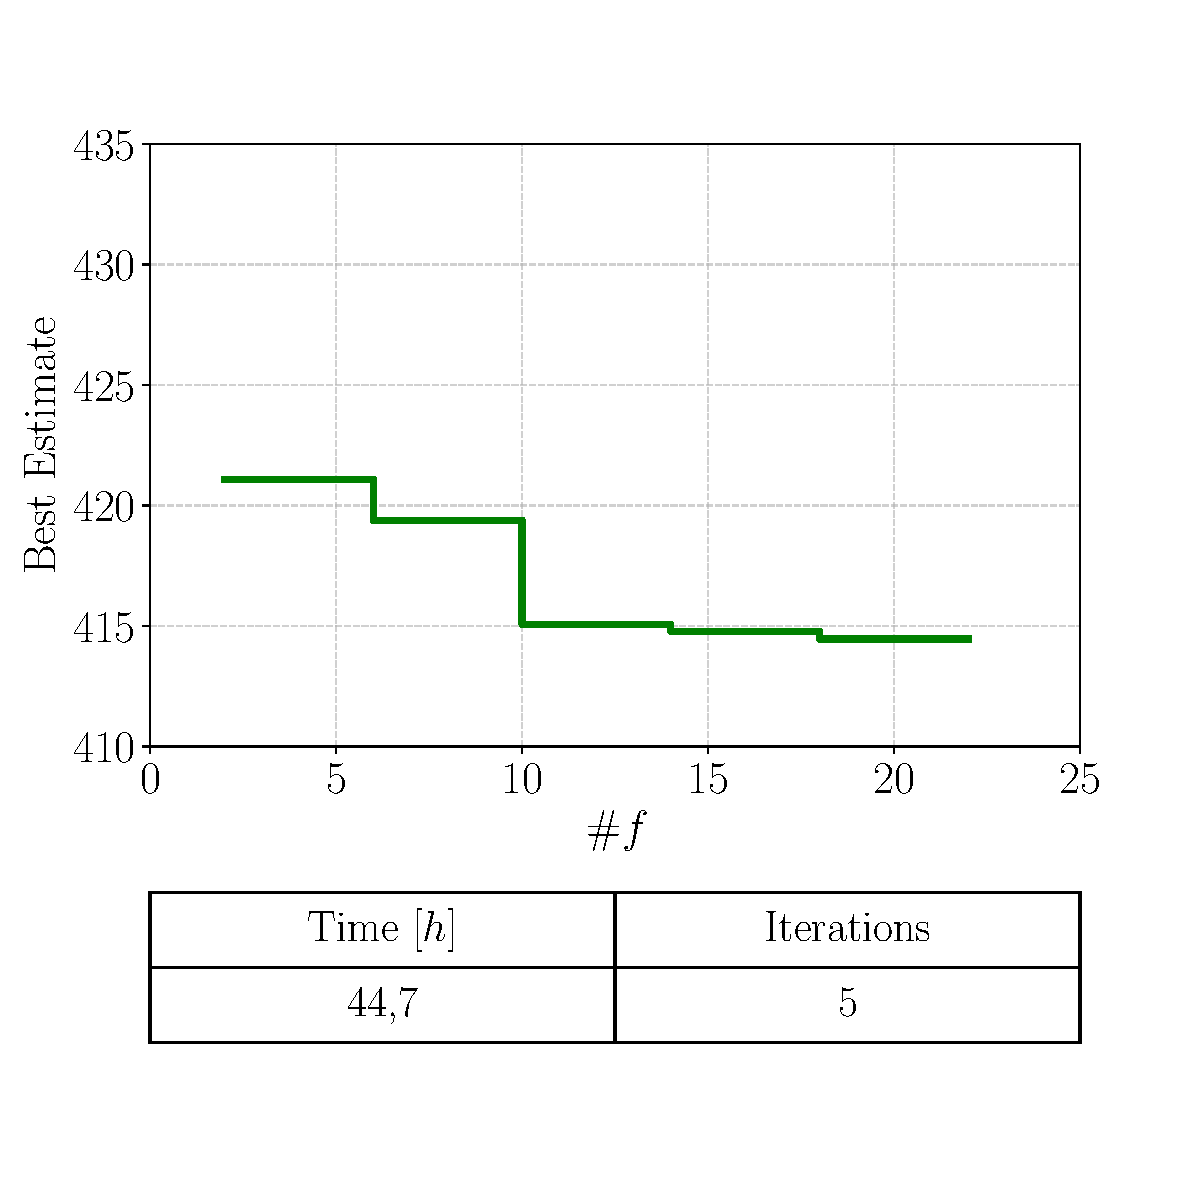
\includegraphics[
		width=1.05\textwidth,
		trim={0mm 25mm 0mm 0mm}, clip
		]{figures/optim_results/nm_tke.pdf}
	\end{subfigure}
	\vspace{2mm}
	\caption{Optimization results for Optimization Setup 2. The left plot compares the optimization result (marked point) with the previously sampled and interpolated objective function $\dot{\gamma}_{\text{max}}^{A}$ as a function of the parameter $o_1$. The right plot demonstrates the convergence of the optimization method, showing the best estimate against the number of objective function evaluations ($\# f$). The table summarizes the total elapsed time of the optimization algorithm (44,7 hours) and the number of iterations of the used method (5).}
\end{figure}
\newpage
\begin{optimproblem}{Basic cylindrical junction ($\dot{\gamma}^{A}_{\text{nw}}$)}
	\vspace{2mm}
	Objective: Minimizing turbulent kinetic energy $\dot{\gamma}^{A}_{\text{nw}}$.
	
	\vspace{2mm}
	Geometrical model:
	\begin{itemize}
		\item Model 1 as described in Section~\ref{mod:model1}.
		\item Optimization parameters: offset $o_1$.
	\end{itemize}
	Constraints:
	\begin{itemize}
		\item Offset constraint: $0{,}0~\text{cm} \leq o_1 \leq 2{,}4~\text{cm}$.
		\item Flow split constraint: $F^{\text{LPA}}_{\text{IVC}} \geq 25~\%$.
	\end{itemize}
	Optimization method:
	\begin{itemize}
		\item MADS method described in Section~\ref{framework}.
	\end{itemize}
	Initial point: $o^{\text{init}}_{1}$ = 0{,}39 cm
	\label{optimprob:3}
\end{optimproblem}

\begin{figure}[H]
	\centering
	\begin{subfigure}{0.47\textwidth}
		\centering
		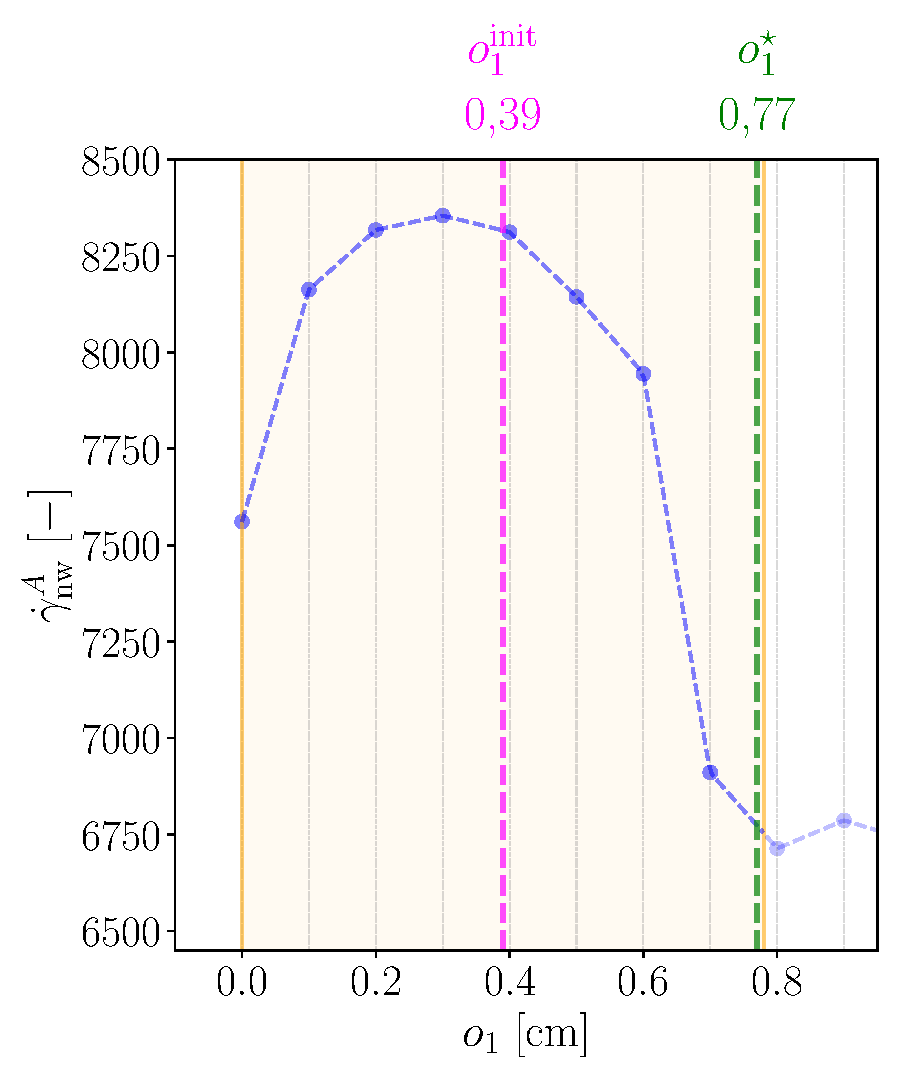
\includegraphics[
		width=\textwidth,
		trim={0mm 0mm 0mm -23mm}, clip
		]{figures/mean_stress_3_interpolated_point.pdf}
	\end{subfigure}\hfill%
	\begin{subfigure}{0.52\textwidth}
		\centering
		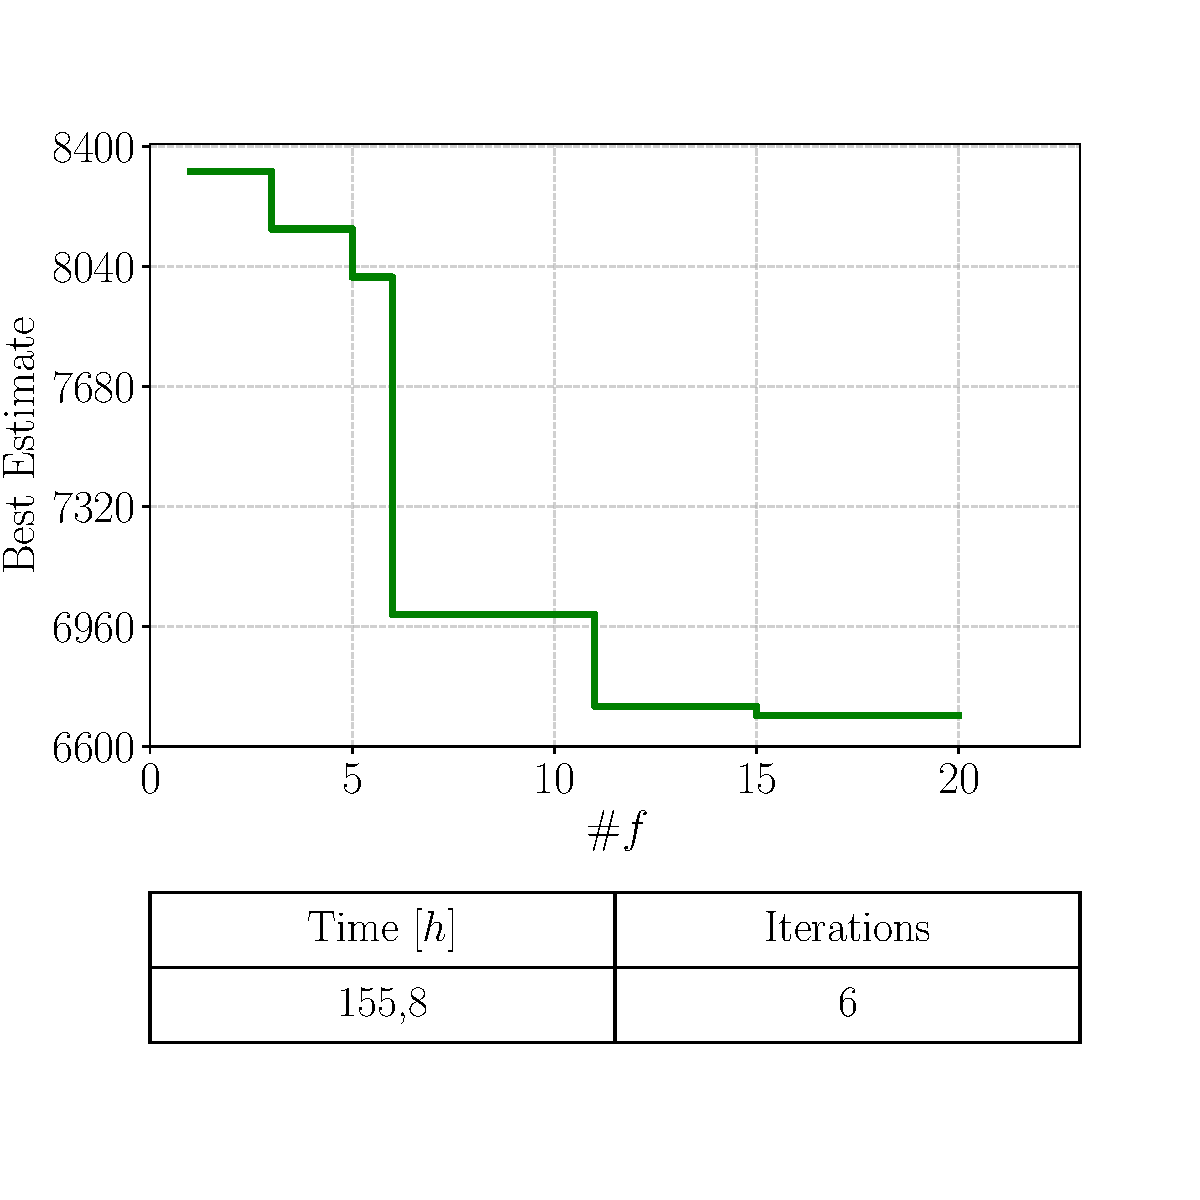
\includegraphics[
		width=1.05\textwidth,
		trim={0mm 25mm 0mm 0mm}, clip
		]{figures/optim_results/mads_sr.pdf}
	\end{subfigure}
	\vspace{2mm}
	\caption{Optimization results for Optimization Setup 3. The left plot compares the optimization result (marked point) with the previously sampled and interpolated objective function $\dot{\gamma}_{\text{max}}^{A}$ as a function of the parameter $o_1$. The right plot demonstrates the convergence of the optimization method, showing the best estimate against the number of objective function evaluations ($\# f$). The table summarizes the total elapsed time of the optimization algorithm (155,8 hours) and the number of iterations of the used method (6).}
\end{figure}
\newpage


\begin{optimproblem}{Basic cylindrical junction ($T^{A}_{\mathrm{turb}}$)}
	\vspace{2mm}
	Objective: Minimizing turbulent kinetic energy $T^{A}_{\mathrm{turb}}$.
	
	\vspace{2mm}
	Geometrical model:
	\begin{itemize}
		\item Model 1 as described in Section~\ref{mod:model1}.
		\item Optimization parameters: offset $o_1$.
	\end{itemize}
	Constraints:
	\begin{itemize}
		\item Offset constraint: $0{,}0~\text{cm} \leq o_1 \leq 2{,}4~\text{cm}$.
		\item Flow split constraint: $F^{\text{LPA}}_{\text{IVC}} \geq 25~\%$.
	\end{itemize}
	Optimization method:
	\begin{itemize}
		\item MADS method described in Section~\ref{framework}.
	\end{itemize}
	Initial point: $o^{\text{init}}_{1}$ = 0{,}39 cm
	\label{optimprob:4}
\end{optimproblem}
\vspace{-5mm}

\begin{figure}[H]
	\centering
	\begin{subfigure}{0.46\textwidth}
		\centering
		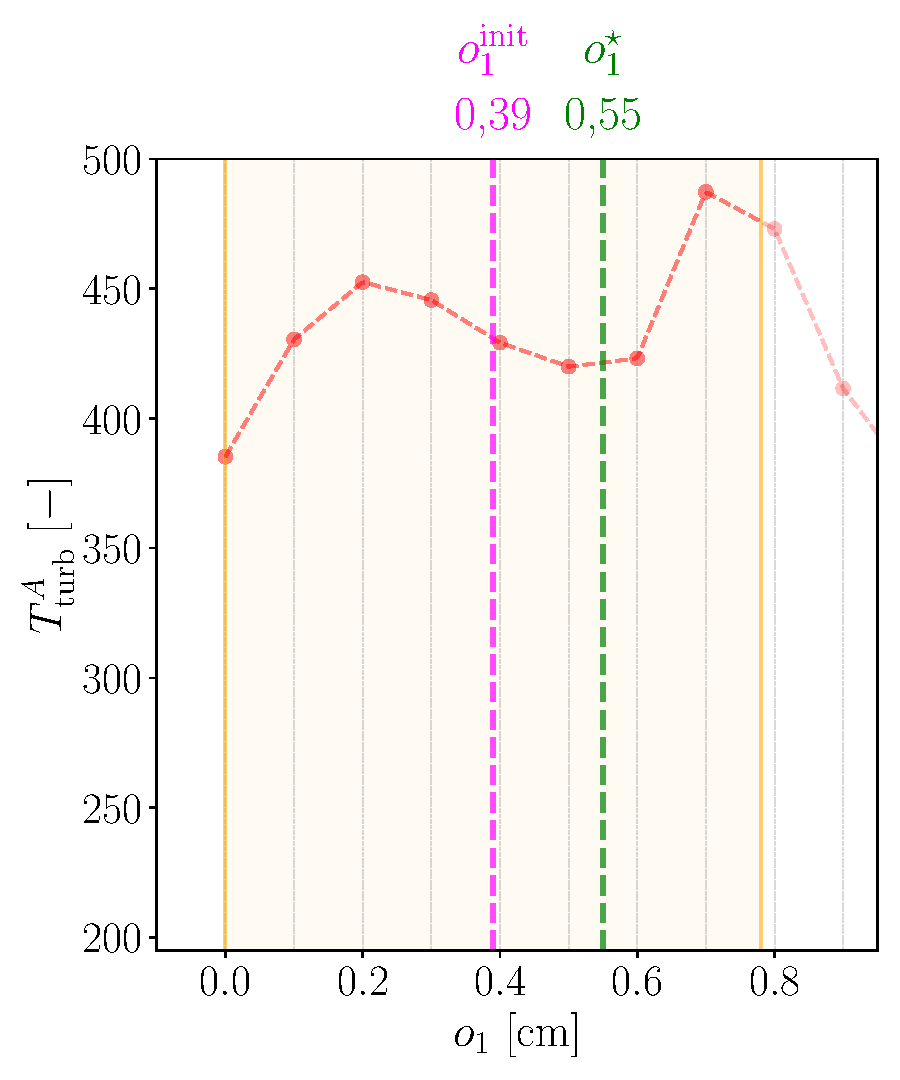
\includegraphics[
		width=\textwidth,
		trim={0mm 0mm 0mm -13mm}, clip
		]{figures/mean_turbulence_kinetic_energy_interpolated_point.pdf}
	\end{subfigure}\hfill%
	\begin{subfigure}{0.52\textwidth}
		\centering
		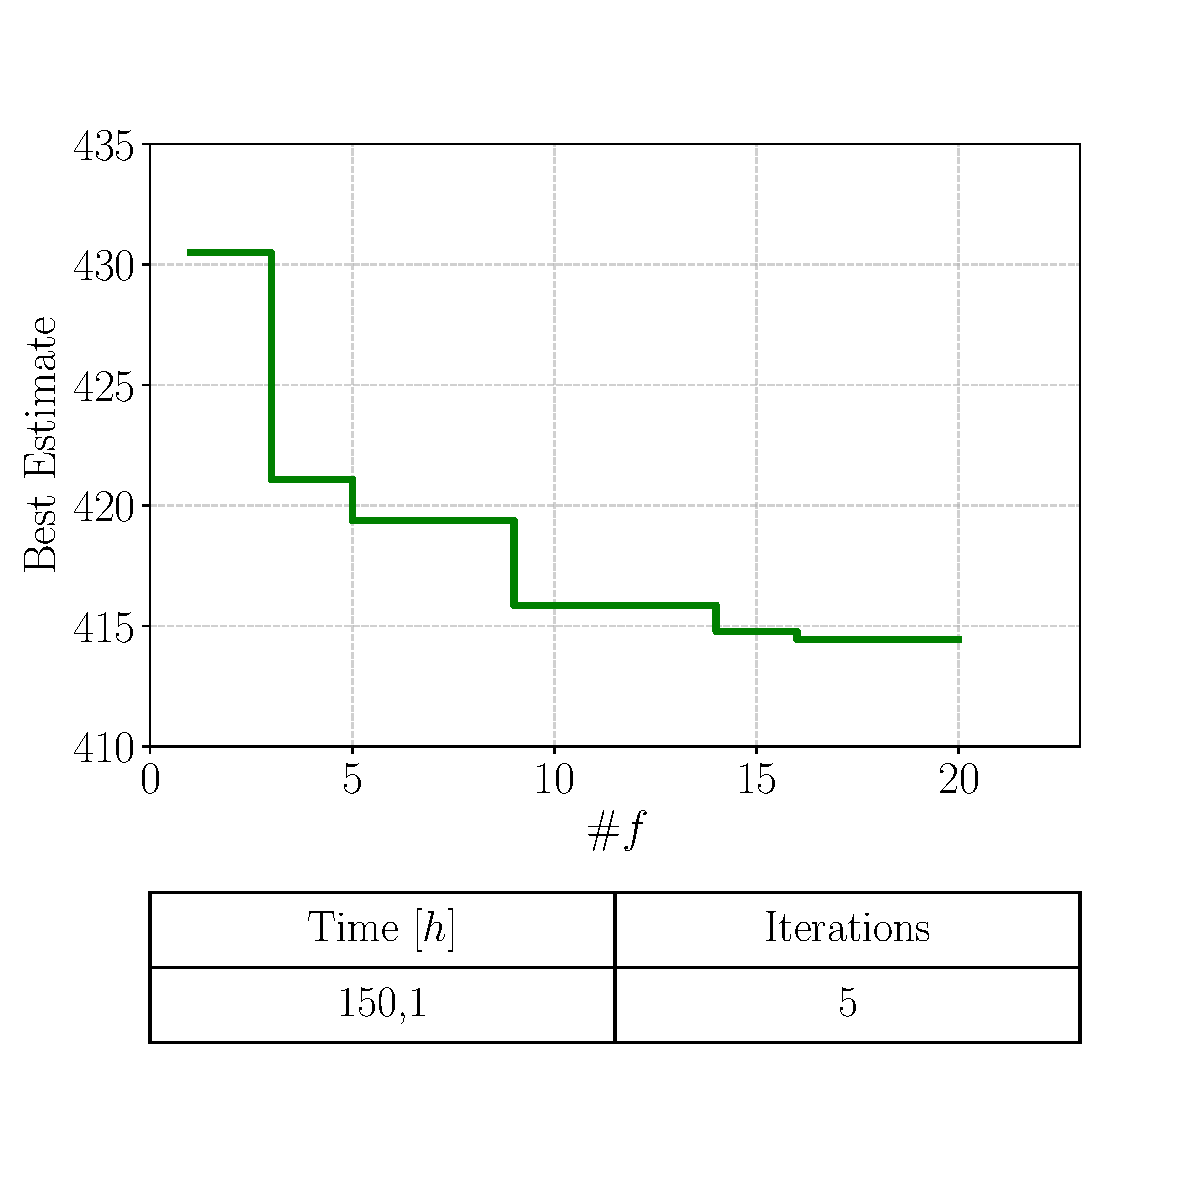
\includegraphics[
		width=1.05\textwidth,
		trim={0mm 25mm 0mm 0mm}, clip
		]{figures/optim_results/mads_tke.pdf}
	\end{subfigure}
	\vspace{2mm}
	\caption{Optimization results for Optimization Setup 4. The left plot compares the optimization result (marked point) with the previously sampled and interpolated objective function $\dot{\gamma}_{\text{max}}^{A}$ as a function of the parameter $o_1$. The right plot demonstrates the convergence of the optimization method, showing the best estimate against the number of objective function evaluations ($\# f$). The table summarizes the total elapsed time of the optimization algorithm (150,1 hours) and the number of iterations of the used method (5).}
\end{figure}
\newpage


